%!TEX root = paper.tex

\section{Introduction} % (fold)
\label{sec:introduction}

Automatic loop invariant inference is a fundamental program analysis problem, 
which is useful in software verification, test-case generation, 
compiler optimization, program understanding, etc. 
In this work, we propose a new approach using machine learning 
to actively learn the loop invariant based on the classification of runtime data. 
By combining selective sampling, support vector machine, 
concolic testing and satisfiability modulo theories, 
we refine the inferred loop invariant after each iteration 
until it converges and proves the property preserved by the loop program. 

Generally, a loop program $P$ can be written in the following form, 
where $\mathit{Pre}$, $\mathit{Cond}$ and $\mathit{Post}$ are boolean conditions, 
and $\mathit{Body}$ is the loop body. 
\[
    P = \{ \mathit{Pre} \} \mathit{while}(\mathit{Cond}) \{ \mathit{Body} \} \{ \mathit{Post} \}
\]
In practice, the pre-condition $\mathit{Pre}$ is often described by 
the specification documents and checking conditions of the program inputs, 
and the post-condition $\mathit{Post}$ is usually specified 
by assertions and exceptions leading to an error state in the program. 
Let $S = \{ x_1 \mapsto v_1, \ldots, x_n \mapsto v_n \}$ represent 
the evaluation function of the program variables $x_1, \ldots, x_n$
and $\mathit{Body}(S)$ stand for their new evaluation after the execution of $\mathit{Body}$, 
the above program means that (1) $\mathit{Pre}$ is the assumption of $S$; 
(2) if the $\mathit{Cond}$ is satisfied by $S$ at an iteration, 
$\mathit{Body}$ will be executed and $S$ will be updated to $\mathit{body}(S)$; 
(3) if the $\mathit{Cond}$ is unsatisfied by $S$ at an iteration, 
the while-loop ends and $S$ should satisfy $\mathit{Post}$. 
To prove the correctness of the above program specification, 
we need to find a loop invariant $\mathit{Inv}$ satisfying the following three conditions. 
\begin{align}
    &S \models \mathit{Pre} 
        &&\Rightarrow && S \models \mathit{Inv} \label{inv:pre} \\
    &S \models \mathit{Inv} \land \mathit{Cond} 
        &&\Rightarrow && \mathit{Body}(S) \models \mathit{Inv} \label{inv:loop} \\
    &S \models \mathit{Inv} \land \neg\mathit{Cond} 
        &&\Rightarrow && S \models \mathit{Post} \label{inv:post}
\end{align}
The goal of this work is developing a method to automatically learn 
the invariant $\mathit{Inv}$ from the loop program and thus prove its correctness. 

% \begin{figure}[t]
%     \begin{center}
%         \begin{subfigure}[b]{0.4\textwidth}
%     \subfloat[A Running Example.]{\scriptsize\begin{verbatim}
%     void P(int x, int y) {
%         assume(x < y);
%         while (x < y) {
%             x = x + 100;
%         }
%         assert(x >= y
%             && x <= y + 99);
%     }\end{verbatim}}
%     \hfill
%     \subfloat[Sampling Areas.]{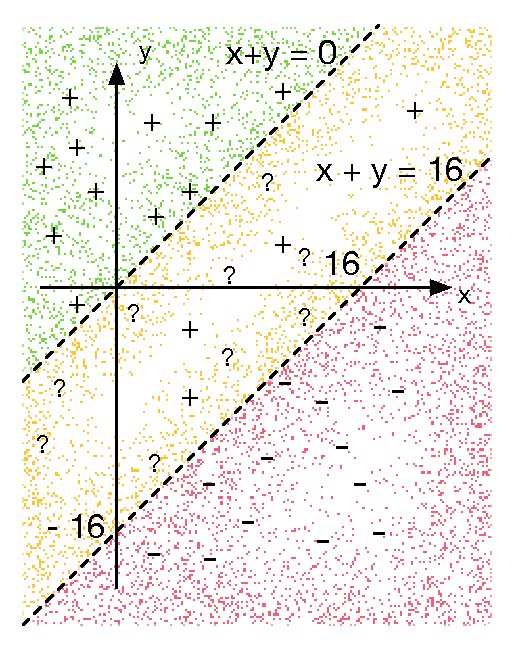
\includegraphics[scale=0.45]{figures/running-sampling.pdf}}
%     \end{center}
%     \caption{A Running Example}
%     \label{fig:running:example}
% \end{figure}

\begin{figure}[t]
    \centering
    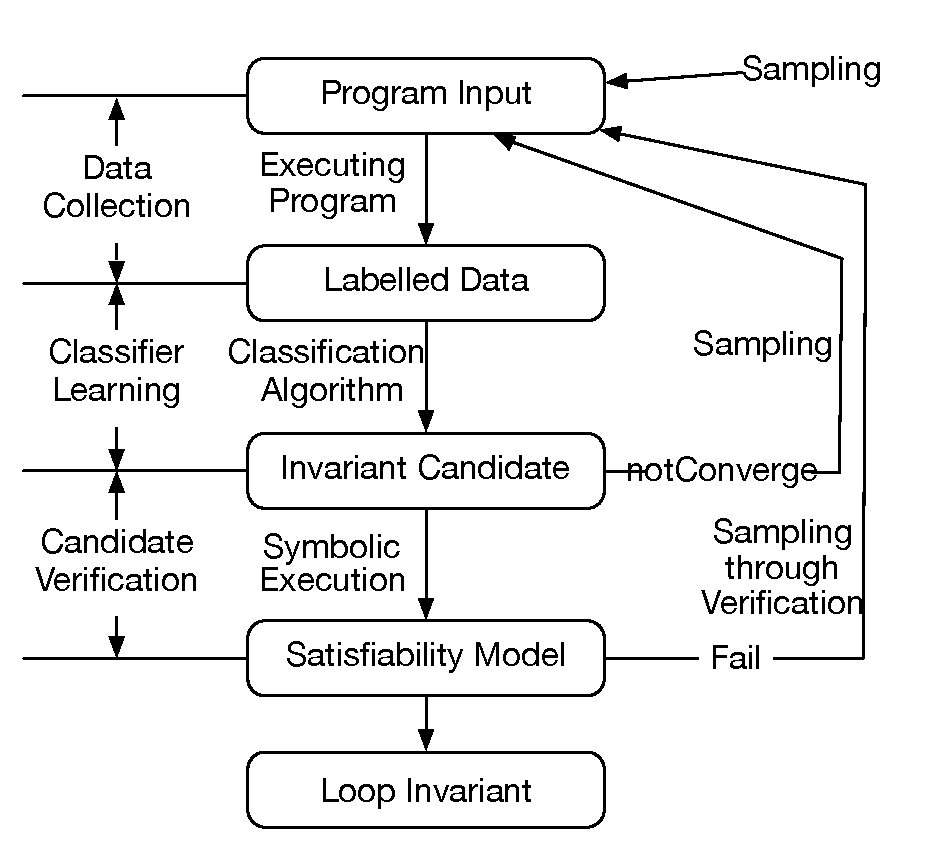
\includegraphics[scale=0.45]{figures/overview.pdf}
    \caption{Loop Invariant Inference Overview}
    \label{fig:overview}
\end{figure}

\medskip\noindent
\textbf{A Running Example}
is shown in Figure~\ref{fig:running:example}. 
The loop program $P$ takes two integers $x$ and $y$ as inputs. 
The assumption $\mathit{Pre}$ requires that $x < y$, 
which is the same as the loop condition $\mathit{Cond}$. 
When $\mathit{Cond}$ is met, 
$x$ is increased by $100$ in each loop iteration. 
Thus, $\mathit{Body}(\{ x \mapsto v \}) = \{ x \mapsto v + 100 \}$. 
Finally, the assertion of $P$ specifies that $y \le x \le y + 99$. 
The correctness of the program specification in Figure~\ref{fig:running:example} 
can be proven by checking the three conditions 
(\ref{inv:pre}), (\ref{inv:loop}) and (\ref{inv:post}) above 
with a loop invariant $\mathit{Inv} = x \le y + 99$. 
We use this running example in the following 
to illustrate different stages of our invariant reference method. 

\medskip\noindent
\textbf{Overview.}
Our approach take the invariant reference as a refinement process 
based on iterations of sampling, classification and verification 
as shown in the Figure~\ref{fig:overview}. 
\begin{itemize}
    \item 
    % (1)
    In the \textbf{Sampling} stage (see Section~\ref{sec:sampling}), 
    we execute the loop program $P$ based on three kinds of sampling sources: 
    random sampling, selective sampling and counter-example sampling. 
    Then, we execute $P$ with different samples to record $S$ in every loop iteration 
    and label them based on the satisfaction of $\mathit{Pre}$ and $\mathit{Post}$. 
    The regions of different labels can be intuitively shown\footnote{
        The `green' (`yellow' and `red' resp.) areas 
        represent `positive' (`uncertain' and `negative' resp.) samples. 
    } as the areas of different colors in Figure~\ref{fig:running:example}. 
    When an program input can be found such that 
    $\mathit{Pre}$ is $\mathit{true}$ and $\mathit{Post}$ is $\mathit{false}$, 
    we output it as a proof of the program specification error. 
    \item 
    % (2) 
    Based on $S$ and their labels collected in the \emph{sampling} stage, 
    we \emph{actively} learn the loop invariant using machine learning algorithms, 
    e.g., different SVM derivatives, in the \textbf{Classification} stage 
    (see Section~\ref{sec:classification}). 
    When the recently learnt invariant converges to the previously learnt ones, 
    we treat it as a invariant candidate and move to the verification step. 
    Otherwise, we apply selective sampling on the recently learnt invariant 
    to add more samples in the sampling stage. 
    \LL{We prove the termination of this process.}
    \item 
    % (3) 
    When an invariant candidate is found, 
    we check its correctness in the \textbf{Verification} stage (see Section~\ref{sec:verification}). 
    First, we insert the candidate into the loop program and generate all the program execution traces 
    based on concolic testing using KLEE. 
    Then, we verify three loop invariant conditions 
    with respect to all of the program execution traces (i.e., different $\mathit{Body}$) 
    using a SMT solver (e.g., Z3 in this work). 
    If the verification is successful, we claim the correctness of $P$ and output the loop invariant. 
    Otherwise, we add the counter-example from Z3 as a new sample 
    and restart from the \emph{sampling} stage. 
\end{itemize}

\medskip\noindent
\textbf{Contributions.}


% section introduction (end)